\documentclass[stochastic-or.tex]{subfiles}
\usepackage{amsmath} % this is only used to enforce good environment completion in emacs
\externaldocument{stochastic-or}

\loadgeometry{tufte}


\begin{document}

\section{\texorpdfstring{$M^B/M/1$}{MBM1pk} Queue and Rejection Policies}
\label{sec:mxm1-queue:-expected}

Sometimes jobs arrive in batches, rather than as single units.
For instance, when a car or a bus arrives at a fast-food restaurant, a batch consists of the number of people in the vehicle.
When the batches arrive as a Poisson process and the individual items within a batch have exponential service times we use the shorthand $M^X/M/1$ for this queueing model.
Using the renewal-reward theorem we derive expressions for the load, the expected waiting time  $\E W$ in queue and expected number of jobs $\E L$ in the system.

To compute more difficult performance measures such as the loss probability $\P{\L>n}$, we need expressions for the stationary distribution $\pi(n)$.
We use level-crossing to derive a recursive scheme, which, when combined with a policy to reject batches, can be used to compute these probabilities.


\newthought{Assume that jobs} arrive as a Poisson process with rate $\lambda$ and each \emph{job} contains multiple \emph{items}.
%Let $A_k$ be the arrival time of job~$k$ and $A(t)$ the number of (job) arrivals up to time~$t$.
Denote by $B_k$ the number of items, i.e., the batch size, of the~$k$th job.
We assume that $\{B_k\}$ is a sequence of iid discrete rvs with common rv~$B$.
We write $S_{k,i}$ for the service time of the~$i$th item of batch~$k$, and assume that $\{S_{k, i}\}$ is a sequence of iid rvs with common rv~$S$, and that the service times of the items are independent of the sizes of the batches.
The utilization is therefore
%\begin{equation*}
$\rho = \lambda \E B \E S$;
%\end{equation*}
As always we require that $\rho<1$.


An arriving job joins the end of the queue (if present), and once the queue in front of it has been cleared, it moves in its entirety to the server.\sidenote{This is the same batching model as in~\cref{sec:setups-batch-proc}.}
Thus, all items in one batch spend the same time in queue.
Once the batch moves to the server, the server processes the items one after another until the batch is finished.
Write $\QQ^B$ for the number of batches in queue and $\Ls^B$ for the number of items (if any) at the server.


Observe that the average time $\E{\W^{B}}$ a batch spends in queue is\sidenote{First  the items at the server have to be served, then the ones in queue.}
\begin{equation*}
  \E{\W^B} =  \E{\Ls^B}\E S + \E{\QQ^B} \E B \E S.
\end{equation*}
But since $\E{\Ls^B} + \E{\QQ^B} \E B = \E \L$,
\begin{align*}
  \E{\W^B} &=  \E\L \E S = \E{\W},
\end{align*}
where $\E W$ is the average time an \emph{item} spends in queue.
We conclude that the average time a job spends in queue is the same as the average time an item spends in queue.

Substituting the equality\sidenote{Little's law}  $\E{\QQ^B} = \lambda \E{\W^B}$  in the above yields
\begin{align}\label{eq:96}
\E W =  \E{\W^B} &= \frac{\E{\Ls^B}}{1-\rho}\E{S}.
\end{align}
It remains to find an expression for $\E{\Ls^B}$.

For this we can use the renewal reward theorem.
With the notation for the proof of Little's law as inspiration, define $Y(t) := \int_0^t \Ls^B(s) \d s$, so that $Y(t)/t$  is the time-average number of items at the \emph{server}.
By taking $D_k$ as the departure time of the~$k$th batch, let $X_k = Y(D_k)-Y(D_{k-1})$.
Suppose the~$k$th job has batch size $B_{k}$, then
  \begin{align*}
    X_k|B_{k} &= \int_{D_{k-1}}^{D_k} \Ls^B(s) \d s
    = B_{k} S_{k,1} + (B_{k}-1)S_{k,2} + \cdots + S_{B_{k}, B_{k}}.
  \end{align*}
Using Adam's law\sidenote{$\E{\E{Y|X}} = \E Y$.}, and that the $S_{k,i}$ are iid,
\begin{align*}
    \E{X_k | B_k} &= B_{k}\E S + (B_{k}-1)\E S + \cdots \E S = B_{k}(B_{k}+1)/2 \cdot \E S, \\
    \E{X_k} & = \E{\E{X_k| B_k}} = \E{\frac{B(B+1)}2} \E S =    \frac{\E{B^2}+\E B}2 \E S,
\end{align*}
as $B_{k}\sim B$, i.e., distributed as the common rv~$B$.
Since $Y=\lim_{t\to\infty} Y(t)/t = \E{\Ls^{B}}$, $Y=\lambda X$, $\lambda = \delta$, and $\rho=\lambda \E B \E S$, we obtain
\begin{align}\label{eq:17}
  \E{\Ls^B} &= \lambda \frac{\E{B^2}}2\E S + \frac\rho 2. % = \frac{\E{B^2}}{2\E B}\rho + \frac\rho 2
\end{align}
We can brush this up by realizing that
\begin{align*}
\frac{\E{B^2}}{(\E{B})^2}
  =\frac{\E{B^2}-(\E B)^2 + (\E B)^2}{(\E{B})^2}
= \frac{\V B + (\E B)^2}{(\E B)^2}= C_s^2+1.
\end{align*}
where $C_s^2 = \V B/ (\E B)^{2}$ is the SCV of the batch size distribution.  Substituting this into the above gives the final result
\begin{equation}\label{eq:43}
\E{\W} =
\frac{1+C_s^2}2 \frac{\rho}{1-\rho} \E B \E S + \frac12\frac\rho{1-\rho} \E S.
\end{equation}

This formula is an important result.
It tells us that the load increases when the load increases or the variability $C_{s}^{2}$ of the batch size increases, but also when $\E B \E S$ increases (even when the utilization $\rho$ remains the same). As such, it gives us the most important clues about  what we should try to change if we want to improve a queueing system.

\newthought{Rather than using} the time an entire batch spends at the server, as in the above use of the renewal-reward equation, we can
concentrate on the expected time spent by single items at the server.
This will provide us with a simple expression for $\P{\Ls=i}$, from which we can also derive~\cref{eq:17}.

If $\Ls(t)$ is the number of items (of the batch in service) at the server at time~$t$, then $Y_i(t) = \int_0^t \1{\Ls(s)=i} \d s$ is the total time there are~$i$ items at the server.
By sampling $Y(\cdot)$ at departure times $\{D_k\}$, we see that
\begin{align*}
X_k = Y_i(D_k) - Y_i(D_{k-1}) = S_{k,i} \1{B_{k} \geq i},
\end{align*}
where $S_{k,i}$ is the service time of the~$i$th remaining item of the batch.
Since the $\{S_{k, i}\}$ are iid\ with $\E{S_{k,i}} = \E S$, and the $\{B_k\}$ are iid and independent of the service times of the items, we obtain
 \begin{equation*}
X = \lim_{n\to\infty} \frac{1}{n}\sum_{k=1}^n S_{k,i} \1{B_{k} \geq i} = \E{S \1{B\geq i}} = \E S G(i-1),
 \end{equation*}
since\sidenote{Recall: $\P{A} := \E{\1{A}}$.} $G(i-1) = \E{\1{B\geq i}} = \P{B> i-1}$ is the survivor function of~$B$.
Since, by construction, $Y_i(t)/t \to \P{\Ls=i}$,   we use the renewal reward theorem and rate stability, $\delta = \lambda$, to conclude that
 \begin{align*}
 \P{\Ls = i} &= \lambda \E{S} G(i-1) = \rho \frac{G(i-1)}{\E B}, \\
 \E{\Ls} &= \sum_{i=0}^\infty i \P{\Ls=i} = \frac{\rho}{\E B} \sum_{i=1}^\infty i G(i-1).
\end{align*}
Simplifying\sidenote{\cref{ex:ER}}  the summation yields~\cref{eq:43}.


\begin{figure}[t]
 \centering
 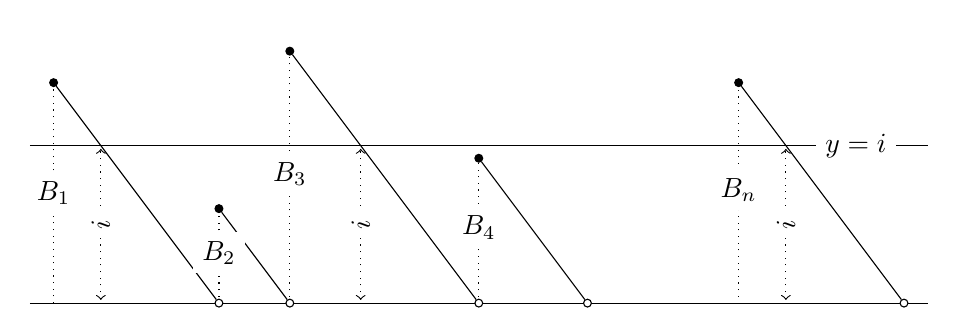
\begin{tikzpicture}[yscale=0.8,xscale=0.6,
 open/.style={shape=circle, fill=white, inner sep=1pt, draw, node contents=},
 closed/.style={shape=circle, fill=black, inner sep=1pt, draw, node contents=}]

 % y = zero line
 \draw (-0.5, 0) -- (18.5, 0);
 % level crossing
 \draw (-0.5, 2.5) -- (18.5, 2.5)
 %node[pos=0.65, fill=white, above] {$\sum_{k=1}^n \1{B_k \geq i}$}
 node[pos=0.92, fill=white] {$y=i$};


 \draw node (c1) at (0,3.5) [closed, label={}]
 node (c2) at (3.5,0)[open, label={}]
 (c1) to (c2);
 \draw[dotted] (0,0) -- (0,3.5) node[midway, fill=white] {$B_1$};
 \draw[dotted, <->] (1, 0.05) -- (1, 2.45) node[fill=white, midway, rotate=90] {$i$};


 \draw node (c1) at (3.5,1.5) [closed, label={}]
 node (c2) at (5,0)[open, label={}]
 (c1) to (c2);
 \draw[dotted] (3.5,0.1) -- (3.5,1.5) node[midway, fill=white] {$B_2$};

 \draw node (c1) at (5,4) [closed, label={}]
 node (c2) at (9,0)[open, label={}]
 (c1) to (c2);
 \draw[dotted] (5,0.1) -- (5,4) node[midway, fill=white] {$B_3$};
 \draw[dotted, <->] (6.5, 0.05) -- (6.5, 2.45) node[fill=white, midway, rotate=90] {$i$};

 \draw node (c1) at (9,2.3) [closed, label={}]
 node (c2) at (11.3,0)[open, label={}]
 (c1) to (c2);
 \draw[dotted] (9,0.1) -- (9,2.3) node[midway, fill=white] {$B_4$};

 % end
 \draw node (c1) at (14.5,3.5) [closed, label={}]
 node (c2) at (18,0)[open, label={}]
 (c1) to (c2);
 \draw[dotted] (14.5,0.1) -- (14.5,3.5) node[midway, fill=white ] {$B_n$};
 \draw[dotted, <->] (15.5, 0.05) -- (15.5, 2.45) node[fill=white, midway, rotate=90] {$i$};


 % bottom line
 %\draw[<->] (0, -0.6) -- (18, -.6) node[fill=white, midway] {$\sum_{k=1}^n B_k$};
\end{tikzpicture}

\caption{A batch crosses the line $y=i$ iff it contains at least~$i$ items.
 Thus, during the service of a batch with~$i$ or more items, there is precisely one service of an~$i$-th item.}
 \label{fig:remainingservicetime}
\end{figure}


\newthought{The second task } is to use level-crossing arguments to find a recursive formula for the state probabilities $\{\pi(n)\}$.\sidenote{Note: $n$ means the number of items in the system, not the number of batches.}
For this we need to generalize our earlier level-crossing equation $\lambda p(n) = \mu p(n-1)$ because, at the arrival of a batch containing many items, multiple levels will be up-crossed, see~\cref{fig:levelcrossing}.


\begin{figure}[t]
\centering
\begin{tikzpicture}[scale=1,
 %Define standard arrow tip
 >=stealth',
 %Define style for boxes
 circ/.style={
 circle,
 draw=black,
 thick,
 minimum size=1.cm,
 inner sep=0pt,
 text centered
 },
 % Define arrow style
 pil/.style={
 ->,
 thick,
 shorten <=2pt,
 shorten >=2pt}
]

\draw[dashed, thick] node at (5,-1.5) [below] {level~$n$}
(5,-1.5) -- (5,3);

\node[circ] (n-2) {$n-2$};

%\node[circ, right=of n-2] (n-1) {$n-1$} edge[loop below, thick] node[midway, fill=white] {$\lambda f(0)$} (n-1);
\node[circ, right=of n-2] (n-1) {$n-1$};

\node[circ, right=of n-1] (n) {$ n $}
 edge[pil,<-, bend left=45] node[below] {$\lambda f(1)$} (n-1.south east);
\node[circ, right=of n] (n+1) {$n+1$}
 edge[pil,bend left=45] node[midway, fill=white] {$\mu$} (n.south east);
\node[above=of n+1] (inf) {}
 edge[pil, <-, bend right=45] node[midway, fill=white] {$\lambda G(0)$} (n.north east)
 edge[pil, <-, bend right=45] node[midway, fill=white] {$\lambda G(1)$} (n-1.north east)
 edge[pil, <-, bend right=45] node[midway, fill=white] {$\lambda G(2)$} (n-2.north east)
;
\end{tikzpicture}

\caption{When $L(t)=n$, the arrival of any batch crosses level~$n$ from below, but when $L(t)=n-1$, only a batch larger than~$1$ ensures a crossing of level~$n$, and so on.} \label{fig:levelcrossing}
\end{figure}

The down-crossing rateof level~$n$ is easy: since items are still served one-by-one, we have $\mu \pi(n+1)$.

For the upcrossings of level~$n$ we should consider batch arrivals that see~$m\leq n$ items in the system.
Since jobs arrive at rate $\lambda$, PASTA implies that $\lambda \pi(m)$ is the arrival rate of jobs that see~$m$ upon arrival; in other words, the process is thinned with a fraction $\pi(m)$.
Next, when an arriving job sees~$m$ in the system, and level~$n$ has to be up-crossed, the batch size of this job must contain more than $n-m$ items.
The rate at which such jobs arrive must be $G(n-m)\pi(m)\lambda$ as $G(n-m)$ is the probability that the job size is larger than $n-m$.
%As a further consequence of PASTA, the arrival process $\{N(u), u\geq t\}$ is independent of $\{L(s), s< t\}$, hence the thinned process is also Poisson.
Noting that the batch sizes are independent of the arrival times, we obtain yet again a Poisson process, but with rate $\lambda \pi(m) G(n-m)$.
Finally, to the compute rate at which level~$n$ is upcrossed, we merge all these thinned Poisson processes into a new Poisson process with rate $\lambda \sum_{m=0}^n \pi(m) G(n-m)$.

As by level-crossing, the up-crossing and down-crossing rates must match,
\begin{equation}\label{eq:42}
\lambda \sum_{m=0}^n \pi(m) G(n-m) = \mu \pi(n+1).
\end{equation}
It is an important check\sidenote{~\cref{ex:73}} to retrieve \cref{eq:43} from the expression $\E\L = \sum_{n} n \pi(n)$ and Little's law.
%At the end of this section, we provide some further details for the interested reader.

\newthought{It is left} to find the normalization constant.
This, however, is not possible in general because ~\cref{eq:42} does not lead to a closed form expression for $\pi(n)$.\sidenote{Compare~\cref{eq:23}.}
A simple and sensible way out is to circumvent the problem altogether by blocking demand above some level~$M$.
There are three common policies to decide which items in a batch to accept.
\begin{enumerate}
\item Complete acceptance: accept all batches that arrive when the system contains~$K$ or fewer items, and reject the entire batch otherwise.\sidenote{~\cref{ex:9}}
\item Partial acceptance: accept whatever fits of a batch, and reject the rest.\sidenote{~\cref{ex:45}}
\item Complete rejection: if a batch does not fit entirely into the system, it will be rejected completely.\sidenote{~\cref{ex:l-156}}
\end{enumerate}
In the exercises we will derive recursions similar to~\cref{eq:42} by which we can obtain $\{\pi(n)\}$.
Since the recursions stop after some level~$M$, there is a finite number of recusions, hence we can solve them numerically without much problems.


\begin{truefalse}
Claim:   Little's Law informs us that in the $M^{B}/M/1$ queue, the expected number of items in queue satisfies $\E{\QQ}=\lambda\E{W}$.
    \begin{solution}
        True.
    \end{solution}
\end{truefalse}

\begin{truefalse}
    For an $M^B/M/1$ queue we know that:
    $$
    \E{W}=\frac{1+C_s^2}{2}\frac{\rho}{1-\rho}\E{B}\E{S}+\frac{1}{2}\frac{\rho}{1-\rho}\E{S}.
    $$
    Suppose that $\V B = 0$.
    Claim: this formula implies that if the batch size increases, but $\E S$ decreases such that $\rho$ remains the same, the expected waiting time becomes smaller.

    \begin{solution}
        True. $\V B = 0 \implies C_{s}^{2} = 0 \implies$ the first term on the RHS does not change when $\rho$ remains constant. The second term does become smaller.
    \end{solution}
\end{truefalse}

\begin{truefalse}
Suppose the time to process an item has an exponential distribution.
Claim: the interarrival times at which individual items arrive at an $M^B/M/1$ queue are exponentially distributed.
    \begin{solution}
        False. Jobs come in batches, hence, multiple items can arrive at the same time, implying that the interarrival distribution is no longer exponential.
    \end{solution}
\end{truefalse}

% \begin{truefalse}
% Consider the $M^B/M/1$ queue with partial acceptance: the system can contain at most $K$ jobs, so that when a batch arrives, accept whatever fits in the queue, and reject the rest.
% Claim: The level-crossing equations are as follows:
%  \begin{equation*}
%  \mu \pi(n+1) = \lambda \sum_{m=0}^n \pi(m) G(n-m),
%  \end{equation*}
%  for $n=0,1,\ldots, K-1$, where $G(n-m)=\P{B>n-m}$ is the survivor function of the random batch size $B$.
% \begin{solution}
% True.

% Here is a variation of the question. Claim: for the $M^B/M/1$ queue the level crossing equations are given by
% $$
% \lambda\sum_{i=0}^n \pi(i)\sum_{j=n-i+1}^\infty\mathbb{P}(B=j)=\mu\pi(n+1).
% $$
% This claim is true, btw.
% \end{solution}
% \end{truefalse}

% \begin{truefalse}[5.5]
% For the $M^X/M/1$ queue, if $B_r$ is the number of items of the batch currently at the server and $\QQ_{b}$ the number of batches in queue, then
% \begin{equation*}
%  \E{L} = \E{\QQ_{b}}\E B + \E{B_r}.
% \end{equation*}
% \begin{solution}
% True.
% \end{solution}
% \end{truefalse}

\begin{truefalse}
Claim: this code correctly implements an $M^{B}/M/1$ queue with complete rejection.
\begin{minted}{python}
def complete_rejection(K):
    pi, n = {}, 0
    pi[0] = 1
    while n < K:
        pi[n + 1] = sum(
            pi[m] * (S.sf(n - m) - S.sf(K - m)) for m in range(n)
        )
        pi[n + 1] *= rho
        n += 1
    return RV(pi)
\end{minted}
\begin{solution}
    False. The range over $m$ should include $n$; now it runs up to (but not including) $n$.
\end{solution}
\end{truefalse}



\begin{exercise}\label{ex:64}
A company operates a machine that receives batches of various sizes.
Management likes to know how a reduction of the variability of the batch sizes would affect the average queueing time.
%\marginpar{Of course, it is up to management to decide whether such reductions outweigh any efforts to reduce the variation in batch sizes.}
Suppose, for the sake of an example, that the batch size $\P{B=1} = \P{B=2} = \P{B=3} = 1/3$.
Batches arrive at rate $\lambda = 1/h$.
The average processing time for an item is $25$ minutes.
Compute by how much $\E\L$ would decrease if $B\equiv 2$.
\begin{solution}

 Start with the simple case.
 $B\equiv 2 \implies \V B=0 \implies C_s^2 = 0$,  $\rho=\lambda \E B \E S = 1\cdot 2 \cdot 25/60 = 5/6$. Hence,
 \begin{equation*}
 \E{\L} = \frac 12 \frac{5/6}{1/6} 2 + \frac 12 \frac{5/6}{1/6} = 5 + \frac52.
 \end{equation*}

Now the other case. $\E{B^2} = (1+4+9)/3 = 14/3$. Hence, $\V B=14/3 - 4=2/3$. Hence,
$C_s^2= \frac 16$.
And thus,
 \begin{equation*}
 \E{\L} = \frac {1+1/6}2 \frac{5/6}{1/6} 2 + \frac 12 \frac{5/6}{1/6} = \frac76 5 + \frac 52.
 \end{equation*}

 The ratio between $\E{\L}$ is $10/9$:  the average waiting time can be reduced by about  10\%  by working in fixed batch sizes.
\end{solution}
\end{exercise}


% \begin{exercise}
% Show that~\cref{eq:43} reduces to the expression for $\E W$ for the $M/M/1$ queue.
% \begin{hint}
% For the $M/M/1$ queue, we have that $B\equiv 1$, i.e., constant. % Why does this imply that $C_s^{2} = 0$?
% \end{hint}
% \begin{solution}
% $B\equiv 1 \implies \V B = 0 \implies C_{s}^{2} =0$ and $\E B = 1$. Filling the formula for $\E S$ is now trivial.
% \end{solution}
% \end{exercise}

% \begin{exercise}\label{ex:l-172}
%  Show
% \marginpar{Relate this to Sakasegawa's formula.}
% that $\E{\W(M^B/M/1)} \geq \E{\W(M/M/1)}$ even when the loads are the same.
%  What do you conclude?
% \begin{hint}
% Use~\cref{eq:96} and that $\V B \geq 0$.
% \end{hint}
% \begin{solution}
% Use \cref{eq:17} to see for the $M/M/1$ queue that $\E{\Ls^{B}} = \rho$ (because for the $M/M/1$ queue, $B\equiv 1$, hence $\E{B^{2}} = \E{B} = 1$(. Again using \cref{eq:17} for the batch queue,
%  \begin{equation*}
%  \frac{\E{\W(M^B/M/1)}}{\E{\W(M/M/1)}} = \frac{\E{\Ls(M^B/M/1)}}{\E{\Ls(M/M/1)}} = \frac{\E{\Ls(M^B/M/1)}}{\rho} =
% \frac{\E{B^2}}{2\E B} + \frac 12.
%  \end{equation*}
%  The RHS is $\geq 1$, because
%  \begin{equation*}
%  \V B \geq 0 \implies \E B^2 \geq (\E B)^2 \implies \frac{\E{B^{2}}}{\E{B}} \geq \E B,
%  \end{equation*}
%  but for any queue $\E B \geq 1$.  Clearly, if variability increases, the average waiting time increases
% \end{solution}
% \end{exercise}


% \begin{exercise}
% Let us write $\E{J_s}$ for the expected time an item spends at the server.
% For the $M/M/1$ it is clear that $\E{J_s} = \E S$.
% It is tempting to believe that $\E{J_s} = 2\E S$ for the $M^2/M/1$ queue, but it is wrong.
% Why?
% \begin{hint}
% Use Little's law and~\cref{eq:17}.
% \end{hint}
% \begin{solution}
% In \cref{eq:17}, $\E{L_S^B} = \rho$ when $B\equiv 1$, but not if $\P{B>1} > 1$.
% \end{solution}
% \end{exercise}



\begin{exercise}\label{ex:l-168}
Compute $\E\L$ for the $M^{B}/M/1$ queue when~$B$ is geometrically distributed with $\E B = 1/p$.
Check that if $\E B =1$ the $M/M/1$ queue results.
\begin{hint}
$\P{B=k}=q^{k-1}p$ with $q=1-p$. Look up the expectation and variance of a geometric rv.
\end{hint}
\begin{solution}
Filling the formula for $\E W$,
 \begin{align*}
 \E B &= \frac 1 p, &  \V B &= \frac1{p^2}-\frac1p, &  C_s^2&= \frac{\V B}{(\E B)^2} = p^2 \left(\frac1{p^2}-\frac1p\right)=1-p, &
 (1+C_s^2)/2 &= 1-p/2,
\end{align*}
\begin{equation*}
\E \L =
\left(1-\frac p2\right) \frac\rho{1-\rho} \frac 1 p + \frac12\frac\rho{1-\rho}
=\frac\rho{1-\rho} \frac 1 p.
\end{equation*}
For the $M/M/1$ queue, $\E B = 1 \implies p = 1 \implies \E\L=\rho/(1-\rho)$.

% If you can't find the expectation and variance of a geometric rv, then here is the derivation.
%  \begin{align*}
%  M_B(s)
% &= \E{e^{sB}} = \sum_{k=0}^\infty e^{sk} \P{B=k} \\
% &= \sum_{k=0}^\infty e^{sk} p q^{k-1}
% = \frac p q \sum_{k=0}^\infty (q e^s)^k = \frac p q \frac1{1-qe^s},\\
%  \E B &= M_B'(0) = \left.\frac p q \frac q{(1-q e^s)^2}\right|_{s=0}= \frac p{(1-q)^2} = \frac 1 p,\\
%  \E{B^2} &= M_B''(0) = \frac2{p^2} - \frac1p, \\
%  \V B &= \E{B^2} - (\E B)^2 = \frac2{p^2} - \frac1p - \frac1{p^2} = \frac1{p^2}-\frac1p,\\
% \end{align*}
\end{solution}
\end{exercise}


\begin{exercise}\label{ex:45}
 Derive a set of recursions for the $M^B/M/1/K$ queue with partial acceptance.
\begin{solution}
  For the partial acceptance case, any job is accepted, but the system only admits whatever fits.
  As level $n\in {0,1,\ldots,K-1}$ is still up-crossed by any batch of size at least $n-m$ when the system is in state~$m$, the formula for the up-crossing rate is identical to the case without this acceptance policy.
  Hence, $\mu \pi(n+1) = \lambda \sum_{m=0}^n \pi(m) G(n-m)$, for $n=0,1,\ldots, K-1$.

This is the code.
\begin{minted}{python}
import numpy as np

from random_variable import RV

labda, mu = 1, 3
rho = labda / mu
f = {1: 1, 2: 1, 3: 1}
S = RV(f)


def partial_acceptance(K):
    pi, n = {}, 0
    pi[0] = 1
    while n < K:
        pi[n + 1] = sum(pi[m] * S.sf(n - m) for m in range(n + 1))
        pi[n + 1] *= rho
        n += 1
    return RV(pi)


pi = partial_acceptance(5)
print(pi.mean())
\end{minted}

\end{solution}
\end{exercise}



\begin{exercise}\label{ex:9}
 Derive a set of recursions analogous to~\cref{eq:42} to compute $\pi(n)$ for the $M^B/M/1/K$ queue with complete acceptance.
\begin{solution}
 The complete-acceptance policy is actually quite simple. As any
 batch will be accepted when $n\leq K$, the queue length is not
 bounded. Only when the number of items in the system is larger than
 $K$, we do not accept jobs.
 \begin{equation*}
 \mu \pi(n+1) =
 \begin{cases}
 \lambda \sum_{m=0}^n \pi(m) G(n-m), & \text{ for } n\leq K,\\
 \lambda \sum_{m=0}^K \pi(m) G(n-m), & \text{ for } n> K.
 \end{cases}
 \end{equation*}

Use the code of~\cref{ex:45} to get a working example.
\begin{minted}{python}
def complete_acceptance(K):
    pi, n = {}, 0
    pi[0] = 1
    while S.sf(n - K) > 0:
        pi[n + 1] = sum(pi[m] * S.sf(n - m) for m in range(min(n, K) + 1))
        pi[n + 1] *= rho
        n += 1
    return RV(pi)
\end{minted}

\end{solution}
\end{exercise}



\begin{exercise}\label{ex:l-156}
 Derive a set of recursions for the $M^B/M/1/K$ queue with complete rejection.
\begin{solution}
  Suppose a batch of size~$k$ arrives when the system contains~$m$ items.
  When $m+k \leq K$, the batch can be accepted since the entire batch will fit into the queue, otherwise it will be rejected.
  Further, level $n, 0\leq n < K$, can only be crossed when $m+k > n$.
  Thus, for $n=0,\ldots, K-1$,
 \begin{align*}
 \mu \pi(n+1) &= \lambda \sum_{m=0}^n \pi(m) \P{n-m < B \leq K-m} \\
&=\lambda \sum_{m=0}^n \pi(m) [G(n-m)-G(K-m)],
 \end{align*}
 Let us check this for some simple cases.
 First, when $K\to \infty$, then $G(K-m)\to 0$, so we get our earlier result.
 Second, take $n=K$.
 Then $G(n-m)-G(K-m)=0$ for all~$m$, so that the RHS is 0, as it should.
 Third, take $n=0$ and $K=1$, then $\mu \pi(1)= \lambda \pi(0)$.
 This also makes sense.

Use the code of~\cref{ex:45} to get a working example.
\begin{minted}{python}
def complete_rejection(K):
    pi, n = {}, 0
    pi[0] = 1
    while n < K:
        pi[n + 1] = sum(
            pi[m] * (S.sf(n - m) - S.sf(K - m)) for m in range(n + 1)
        )
        pi[n + 1] *= rho
        n += 1
    return RV(pi)
\end{minted}
\end{solution}
\end{exercise}


\begin{extra}\label{ex:6}
 For a nonnegative discrete random variable~$X$, use indicator functions to prove that
 \begin{enumerate}
 \item  $\E X = \sum_{k=0}^\infty G(k)$,
 \item $\sum_{i=0}^\infty i G(i) = \E{X^2}/2 - \E{X}/2$.
 \end{enumerate}
\begin{hint}
Write
For 1: $\sum_{k=0}^\infty G(k) = \sum_{k=0}^\infty \sum_{m=k+1}^\infty \P{X=m}$, reverse the summations. Then realize that $\sum_{k=0}^\infty \1{k<m} = m$. For 2:
$\sum_{i=0}^\infty i G(i) = \sum_{n=0}^\infty \P{X=n} \sum_{i=0}^\infty i \1{n\geq i+1}$,and reverse the summations.
\end{hint}
\begin{solution}
For 1, observe first that $\sum_{k=0}^\infty \1{m>k} = m$, since $\1{m>k}=1$ if $k<m$ and $\1{m>k} = 0$ if $k\geq m$. With this,
\begin{align*}
\sum_{k=0}^\infty G(k)
&= \sum_{k=0}^\infty \P{X>k}
= \sum_{k=0}^\infty \sum_{m=k+1}^\infty \P{X=m} \\
& = \sum_{k=0}^\infty \sum_{m=0}^\infty \1{m>k} \P{X=m}
= \sum_{m=0}^\infty \sum_{k=0}^\infty \1{m>k} \P{X=m} \\
&= \sum_{m=0}^\infty m\P{X=m} = \E X.
\end{align*}
There are some technical details with respect to the interchange of the summations.
Since the summands are positive, this is allowed.

For 2,
\begin{align*}
\sum_{i=0}^\infty i G(i)
&= \sum_{i=0}^\infty i \sum_{n=i+1}^\infty \P{X=n} = \sum_{n=0}^\infty \P{X=n} \sum_{i=0}^\infty i \1{n\geq i+1} \\
&= \sum_{n=0}^\infty \P{X=n} \sum_{i=0}^{n-1}i = \sum_{n=0}^\infty \P{X=n} \frac{(n-1)n}{2} \\
&= \sum_{n=0}^\infty \frac{n^2}{2} \P{X=n} - \frac{\E X}{2}
= \frac{\E{X^2}}{2} - \frac{\E X}{2}.
\end{align*}
\end{solution}
\end{extra}

\begin{extra}\label{ex:ER}
 Show that $\sum_{i=1}^\infty i G(i-1)= ({\E{B^2} + \E B})/{2}$.
\begin{hint}
 Use~\cref{ex:6}.
\end{hint}
\begin{solution}
\begin{equation*}
 \begin{split}
 \sum_{i=1}^\infty i G(i-1)
&=\sum_{i=0}^\infty (i+1) G(i)
=\sum_{i=0}^\infty i G(i) +
\sum_{i=0}^\infty G(i)= (\E{B^2} - \E B)/2 + \E B.
 \end{split}
\end{equation*}
\end{solution}
\end{extra}


\begin{extra}\label{ex:73}
Use~\cref{eq:42}
\marginpar{This is an important check both on \cref{eq:43} and~\cref{eq:42}.}
in $\E{\L} = \sum_{n=0}^\infty n \pi(n)$ to derive~\cref{eq:43}.
\begin{hint}
  Show first that
\begin{equation*}
 \mu \E \L =\mu \sum_{n=0}^\infty n \pi(n) = \lambda \frac{\E{B^2}}2 + \lambda \E B \E \L +\lambda \frac{\E B}2.
\end{equation*}
\end{hint}
\begin{solution}
 We use that $\mu \pi(n) =\lambda \sum_{i=0}^{n-1} \pi(i) G(n-1-i)$ and the results of the exercises of~\cref{sec:mxm1-queue:-expected} to see that
\begin{align*}
 \mu \E \L
 &=\sum_{n=0}^\infty n\, \mu \pi(n), \quad \text{now substitute for $\mu \pi(n)$ the recursion~\cref{eq:42}}, \\
& =\lambda \sum_{n=0}^\infty n \sum_{i=0}^{n-1} \pi(i) G(n-1-i)
 =\lambda \sum_{n=0}^\infty n \sum_{i=0}^\infty \1{i<n} \pi(i) G(n-1-i) \\
& =\lambda \sum_{i=0}^\infty \pi(i) \sum_{n=0}^\infty \1{i<n} n G(n-1-i)
 =\lambda \sum_{i=0}^\infty \pi(i) \sum_{n=i+1}^\infty n G(n-1-i) \\
& =\lambda \sum_{i=0}^\infty \pi(i) \sum_{n=0}^\infty (n+i+1) G(n)
 =\lambda \sum_{i=0}^\infty \pi(i) \left[\sum_{n=0}^\infty n G(n) +(i+1) \sum_{n=0}^\infty G(n)\right] \\
 &=\lambda \sum_{i=0}^\infty \pi(i)\sum_{n=0}^\infty n G(n) +\lambda \E B \sum_{i=0}^\infty \pi(i) (i+1) \\
 &=\lambda \sum_{i=0}^\infty \pi(i) \frac{\E{B^2} -\E B}2 + \lambda \E B (\E \L +1) \\
 &= \lambda \frac{\E{B^2} -\E B}2 + \lambda \E B \E \L +\lambda \E B \\
 &= \lambda \frac{\E{B^2} }2 + \lambda \E B \E \L +\lambda \frac{\E B}2.
\end{align*}
Dividing both sides by $\mu$ and using that $\lambda \E B/\mu = \rho$, we obtain
\begin{equation*}
E \L = \lambda \frac{\E{B^2}}2 \E S + \rho \E \L + \frac\rho2.
\end{equation*}
By bringing $\rho \E \L$ to the LHS, the RHS becomes equal to~\cref{eq:17}.
\end{solution}
\end{extra}


% \newthought{Here we formalize} the above reasoning; you can skip it if you understand the details of level crossing.
% Define
% \begin{equation*}
%  A(m,n,t) := \sum_{k=1}^{A(t)}\1{\L(A_k-) = m}\1{B_k > n-m}
% \end{equation*}
% as the number of jobs up to time~$t$ that see~$m$ in the system upon arrival and have batch size larger than $n-m$.
% From~\cref{fig:levelcrossing} we see that $A(n,m,t)$ counts the number of up-crossings of level~$n$ up to time~$t$.

% As earlier, we are interested in the limit $A(n,m,t)/t$ as $t\to\infty$.
% If we follow the reasoning of~\cref{sec:poisson-arrivals-see}, we obtain by multiplying and dividing,
% \begin{equation}\label{eq:16}
%  \frac{A(m,n,t)}t = \frac{A(t)}t \frac{A(m,t)}{A(t)}\frac{A(m,n,t)}{A(m,t)}.
% \end{equation}
% We already know that $A(t)/t\to\lambda$ and $A(m,t)/A(t)\to\pi(m)$; so, let us  provide  an interpretation for the third term.

% If we fill in the definitions, we get
% \begin{equation*}
%  \frac{A(m,n,t)}{A(m,t)} =  \frac{\sum_{k=1}^{A(t)}\1{\L(A_k-) = m, B_k > n-m}}
% {\sum_{k=1}^{A(t)}\1{\L(A_k-) = m}}.
% \end{equation*}
% In words, this is the fraction of those jobs that see~$m$ in the system upon arrival and have size $> n-m$.
% But recall that we assumed that  $\{B_k\}$  are independent of what jobs see upon arrival.
% Thus, we can just as well count all jobs of size $>n-m$ along a sample path instead of those that see~$m$ upon arrival; in the limit the statistics must be the same. Therefore
% \begin{equation*}
% \lim_{t\to\infty}  \frac{\sum_{k=1}^{A(t)}\1{\L(A_k-) = m, B_k > n-m}}
% {\sum_{k=1}^{A(t)}\1{\L(A_k-) = m}} = \lim_{t\to\infty}
% \frac{\sum_{k=1}^{A(t)}\1{B_k > n-m}}{A(t)}= G(n-m).
% \end{equation*}
% By level-crossing $\left|\sum_{m=0}^n A(m,n,t) - D(n,t)\right| \leq 1$, from which we obtain~\cref{eq:16} by combining this with the above, dividing by~$t$, and taking the limit $t\to\infty$.




\input{trailer}

%%% Local Variables:
%%% mode: latex
%%% TeX-master: t
%%% End:
